%----------------------------------------------------------
\chapter{Разработанные структуры данных}\label{chap3_soft_architecture}
%----------------------------------------------------------
Основной структурой данных, поддерживающей разработанный в разделе \ref{chap2_algorithms} алгоритмы является структура данных <<контейнер выполнения>>. Задача её внутренней логики -- контролировать параллельный обход нескольких ветвей графа и отслеживать их слияние. Помимо прочего это подразумевает выделение и освобождение вычислительных ресурсов для параллельного обхода. Поскольку в общем случае могут применяться различные вычислительные ресурсы (потоки ядер процессора, процессы операционной системы, узлы вычислительного кластера и пр.), было принято решение разработать единый интерфейс структуры <<контейнер выполнения>> без привязки к конкретным ресурсам. Это позволит независимо разрабатывать различные реализации данной структуры для различных режимов параллельного обхода. 

Помимо прочего при проектировании интерфейса структуры данных <<контейнер выполнения>> были задействованы разработанные в рамках курсового проекта по дисциплине <<Модели и методы анализа проектных решений>> структуры данных <<операция с вершиной>> (\textsf{NodeOp}) и <<операция с ребром>> (\textsf{EdgeOp})\cite{TrishinMMAPS2022}.

Интерфейсы спроектированных структур данных были описаны с помощью UML-диаграмм, представленных на рисунке \ref{fig:UMLAll}. Были учтены особенности описания классов на языке C++.

\begin{figure}
    \centering
    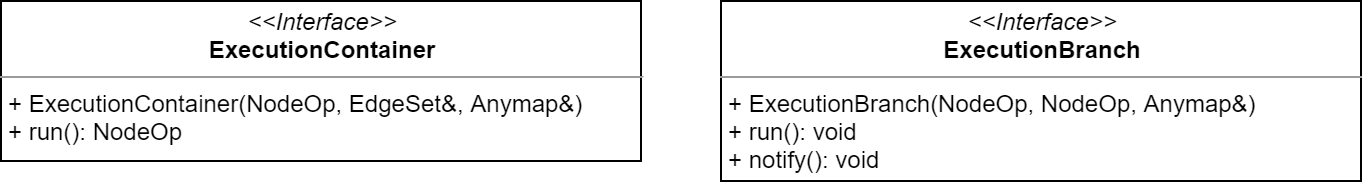
\includegraphics[width=\textwidth]{figures/UML.all.png}
    \caption{UML-диаграммы разработанных структур данных}
    \label{fig:UMLAll}
\end{figure}

Конструктор класса \textsf{ExecutionContainer} соответствует алгоритму, описанному в разделе~\ref{chap2_algorithms}. Метод run выполняет алгоритм, описанный блок-схемой на рисунке~\ref{fig:flowchartExecutionContainer}.

Кроме того, была спроектирован интерфейс структуры <<ветви исполнения>> (\textsf{ExecutionBranch} на рисунке~\ref{fig:UMLAll}). Её задача -- выполнение обхода одной конкретно взятой ветви (метод \textsf{run()}) графовой модели с уведомлением <<контейнера исполнения>> о завершении каждой функции перехода (метод \textsf{notify()}), как того требует алгоритм.

Таким образом, разработанные классы реализуют в себе логику параллельного обхода ветвей графовой модели и хранят данные в соответствии с разработанной процедурой обхода.
%----------------------------------------------------------

